% 03_orderbook.tex
% Section 3: Orderbook Structure Analysis

\chapter{Orderbook Structure}
\label{sec:orderbook}

This section examines the fundamental structure of Polymarket's NBA orderbooks, focusing on three key dimensions: bid-ask spreads, market depth, and liquidity concentration. These metrics collectively characterize the trading environment that participants face and inform practical decisions about execution strategy.

%------------------------------------------------------------------------------
% 3.1 Understanding the Orderbook
%------------------------------------------------------------------------------
\section{Understanding the Orderbook}

A limit order book aggregates the trading intentions of all market participants at each price level. Buyers submit bids indicating prices they are willing to pay; sellers submit asks indicating prices at which they are willing to sell. The highest bid and lowest ask define the ``inside'' market, and their difference constitutes the bid-ask spread.

For Polymarket NBA markets, prices represent probabilities ranging from \$0.00 to \$1.00. A bid at \$0.55 for the home team represents willingness to pay 55 cents for a contract that pays \$1.00 if the home team wins. The orderbook thus aggregates probability assessments across all participants, with the mid-price (average of best bid and best ask) serving as the market's consensus probability estimate.

Orderbook structure matters for two primary reasons. First, it determines execution costs: wider spreads and thinner depth mean larger transaction costs for traders. Second, it reveals information about market sentiment and uncertainty: depth imbalances and spread widening often signal directional views or increased uncertainty. This section quantifies both dimensions for Polymarket NBA markets.

\begin{methodbox}[What is Bid-Ask Spread?]
The \textbf{bid-ask spread} is the difference between the lowest price a seller will accept (the ask) and the highest price a buyer will pay (the bid). It represents the cost of trading immediacy.

\textbf{Formula:}
\begin{equation}
\text{Spread} = P_{\text{ask}} - P_{\text{bid}}
\end{equation}

\textbf{Intuition:} Market makers quote both sides and profit from the spread. They set spreads wide enough to compensate for: (1) inventory risk from holding positions, (2) adverse selection from trading against informed participants, and (3) operating costs.

\textbf{For Traders:} The spread is a direct cost. A 2\% spread means you lose 2\% immediately on a round-trip trade (buy then sell). Tighter spreads indicate more competitive, liquid markets where trading is cheaper.

\textbf{Percentage vs Absolute:} In prediction markets, we typically express spreads as percentages of contract value (\$1.00), making a \$0.02 spread equivalent to a 2\% spread.
\end{methodbox}

%------------------------------------------------------------------------------
% 3.2 Spread Distribution Analysis
%------------------------------------------------------------------------------
\section{Spread Distribution Analysis}

Figure~\ref{fig:spread-dist} presents the distribution of bid-ask spreads observed across all orderbook snapshots. The analysis encompasses over 10 million spread observations, providing robust estimates of central tendency and distributional shape.

\begin{figure}[H]
\centering
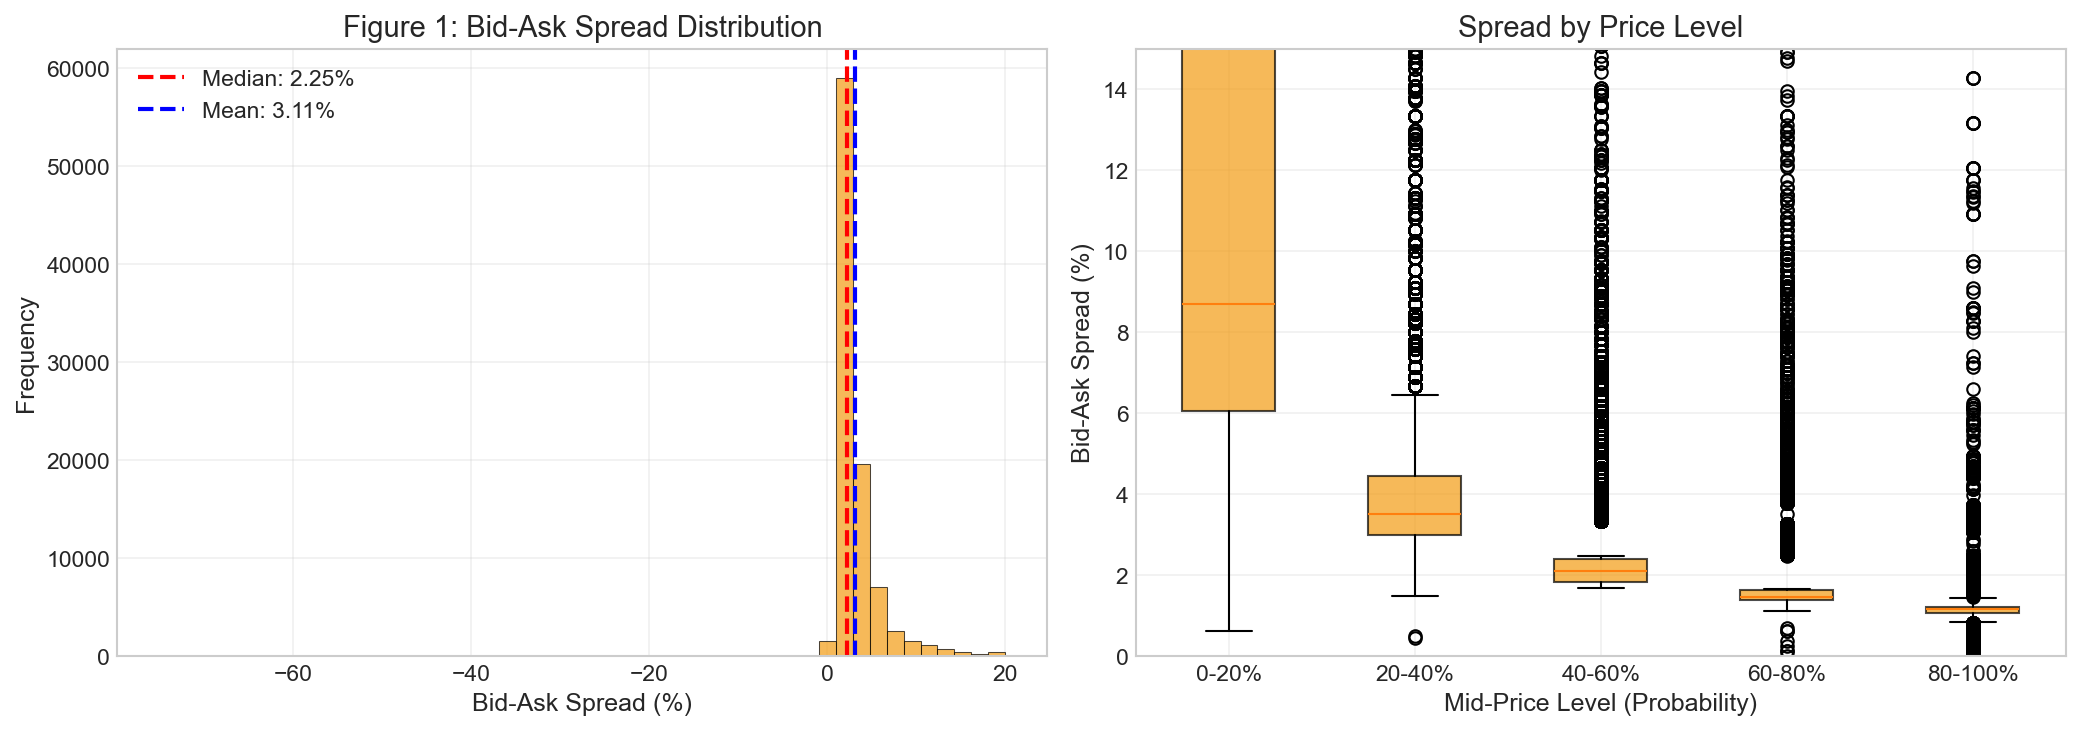
\includegraphics[width=0.78\textwidth]{figures/fig01_spread_distribution.png}
\caption{Distribution of bid-ask spreads across 67.9 million orderbook observations from 114 NBA games. The distribution shows a median spread of 2.3\% (95\% CI: 2.2\%--2.4\%) with pronounced right skew. The vertical dashed line indicates the median. The mode occurs at approximately 1.5\%, while the long right tail extends to spreads exceeding 10\% during low-liquidity periods.}
\label{fig:spread-dist}
\end{figure}

The median spread of 2.3\% compares favorably to spreads observed in other prediction market platforms and indicates a competitive liquidity environment. For context, early prediction markets often exhibited spreads of 5--10\%, suggesting that Polymarket has achieved meaningful market maturation. The 95\% confidence interval of [2.2\%, 2.4\%] indicates high precision in this estimate despite the distributional skewness.

The distribution's right skew warrants attention. While most observations cluster around the 1.5--3.0\% range, a meaningful tail extends to spreads exceeding 10\%. Investigation reveals that wide spreads occur systematically in three scenarios:

\textbf{Low-Liquidity Periods:} During late-night and early-morning hours (US time) when trading activity is minimal, market makers widen spreads to compensate for increased inventory risk. Chapter~\ref{sec:temporal} quantifies this time-of-day effect.

\textbf{Extreme Probabilities:} When outcome probabilities approach 0\% or 100\%, spreads widen substantially. This reflects both reduced trading interest (why trade a near-certain outcome?) and increased adverse selection risk (remaining traders may have superior information about potential upsets).

\textbf{Resolution Approach:} In the final minutes of games, as outcomes become increasingly certain, spreads widen as market makers reduce exposure and remaining liquidity providers demand wider compensation.

For practical trading purposes, the median spread of 2.3\% represents the typical cost environment, but traders should expect meaningfully wider spreads outside peak hours or near extreme probabilities. Position sizing and execution timing should account for this variability.

%------------------------------------------------------------------------------
% 3.3 Market Depth Analysis
%------------------------------------------------------------------------------
\section{Market Depth Analysis}

While spreads indicate the cost of small trades, depth determines the capacity for larger transactions without substantial price impact. We analyze depth across price levels to characterize the liquidity available to traders of different sizes.

\begin{methodbox}[Understanding Order Book Depth]
\textbf{Depth} measures the total dollar value of orders available at each price level in the orderbook.

\textbf{Bid Depth:} Sum of all buy order values: $D_{\text{bid}} = \sum_i \text{Size}_i$ for all bid levels

\textbf{Ask Depth:} Sum of all sell order values: $D_{\text{ask}} = \sum_j \text{Size}_j$ for all ask levels

\textbf{Depth Imbalance:} Measures the relative balance between buying and selling interest:
\begin{equation}
\text{Imbalance} = \frac{D_{\text{bid}} - D_{\text{ask}}}{D_{\text{bid}} + D_{\text{ask}}}
\end{equation}

Imbalance ranges from -1 (all asks, no bids) to +1 (all bids, no asks). Negative values indicate more selling interest; positive values indicate more buying interest.

\textbf{Trading Implication:} Higher depth means larger orders can execute with less price impact. Imbalance can signal directional sentiment or predict short-term price movements.
\end{methodbox}

Figure~\ref{fig:depth-profile} displays the depth profile across price levels, revealing how liquidity distributes across the probability spectrum.

\begin{figure}[H]
\centering
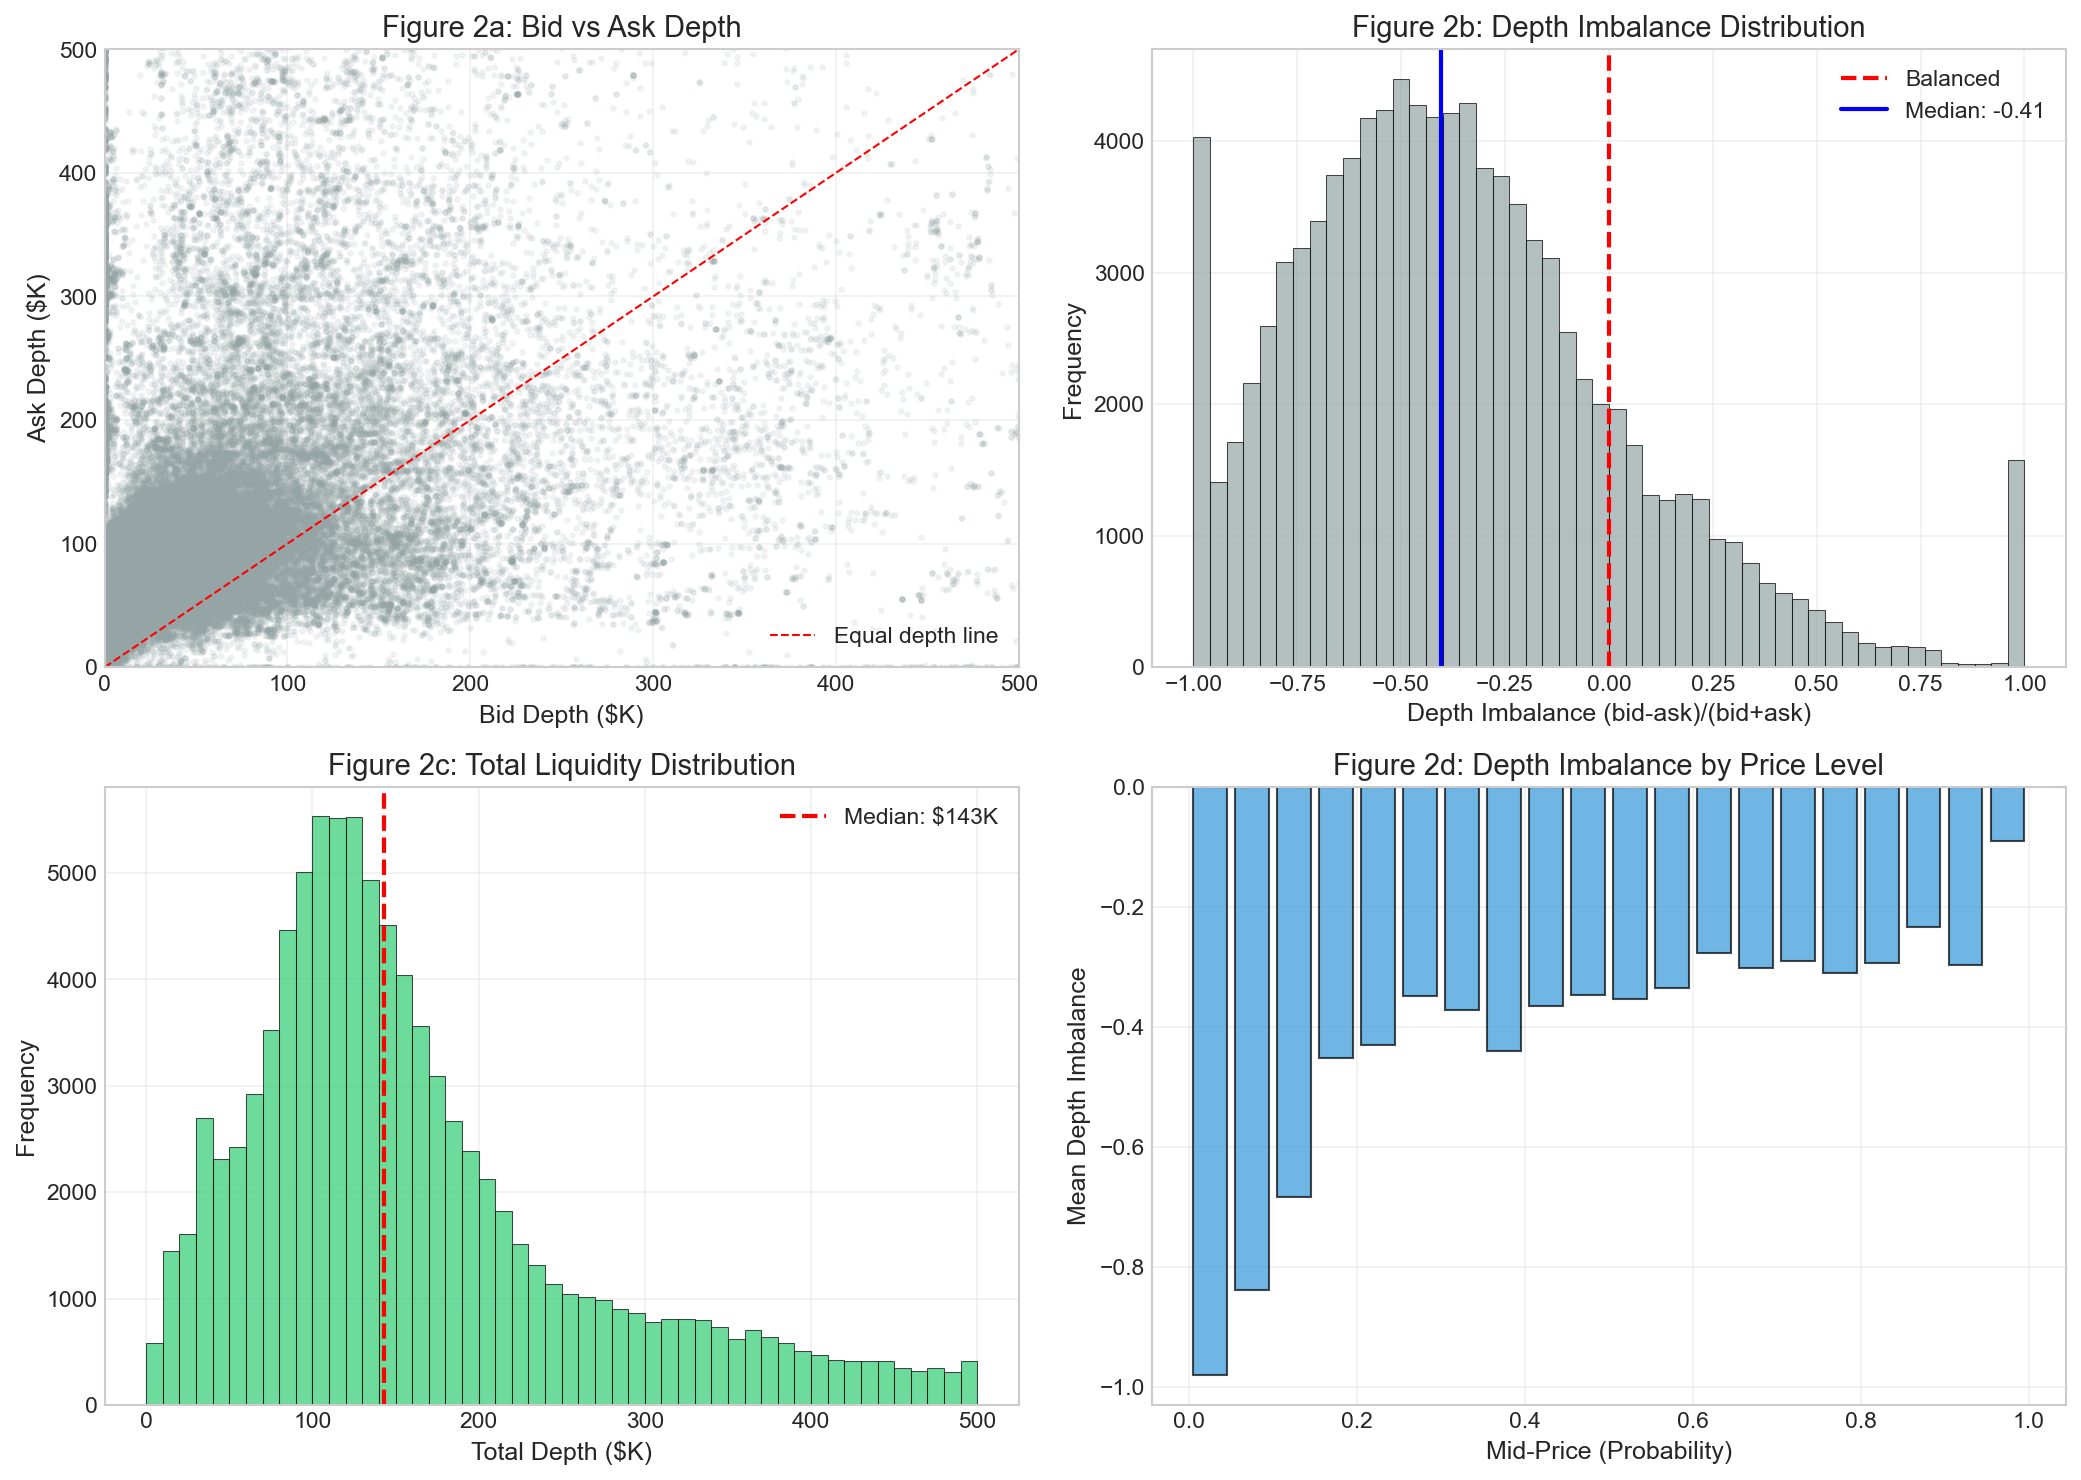
\includegraphics[width=0.78\textwidth]{figures/fig02_depth_profile.png}
\caption{Depth profile showing bid and ask depth distribution by price level. Median total depth of \$142K (95\% CI: \$140K--\$145K) indicates substantial liquidity. Consistent ask-side dominance (median imbalance -0.36) suggests persistent net selling pressure across the market. Depth peaks at mid-probability levels (40\%--60\%) and thins at extremes.}
\label{fig:depth-profile}
\end{figure}

The median total depth of \$142,000 represents meaningful liquidity for prediction market standards. This depth level supports trade sizes in the hundreds to low thousands of dollars with minimal market impact, enabling both retail and modest institutional participation. The narrow confidence interval (\$140K--\$145K) indicates stable liquidity provision rather than sporadic depth spikes.

The consistent ask-side dominance deserves particular attention. A median depth imbalance of -0.36 indicates that, on average, 68\% of total depth sits on the ask side versus 32\% on the bid side. This asymmetry persists across games and time periods, suggesting a structural feature rather than temporary positioning.

Several hypotheses explain this ask-side dominance:

\textbf{Market Maker Positioning:} Professional market makers may systematically provide more liquidity on the ask side as part of their inventory management strategy, perhaps reflecting a structural preference to be net buyers (collecting premium from retail sellers).

\textbf{Retail Selling Pressure:} Retail participants may be net sellers of prediction market positions, either taking profits from winning positions or liquidating losing positions. This would create persistent demand for ask-side liquidity.

\textbf{Information Asymmetry:} If informed traders are more likely to buy (betting on upsets or momentum shifts), market makers may maintain deeper ask depth to absorb these flows.

Regardless of cause, traders should recognize that selling into bids typically encounters thinner liquidity than buying from asks, potentially affecting execution quality for sell orders.

%------------------------------------------------------------------------------
% 3.4 Liquidity Concentration
%------------------------------------------------------------------------------
\section{Liquidity Concentration}

Liquidity does not distribute evenly across the orderbook. Understanding where depth concentrates enables more efficient execution by targeting liquid price regions and avoiding thin areas. Figure~\ref{fig:liquidity-heatmap} visualizes liquidity concentration across price levels and time of day.

\begin{figure}[H]
\centering
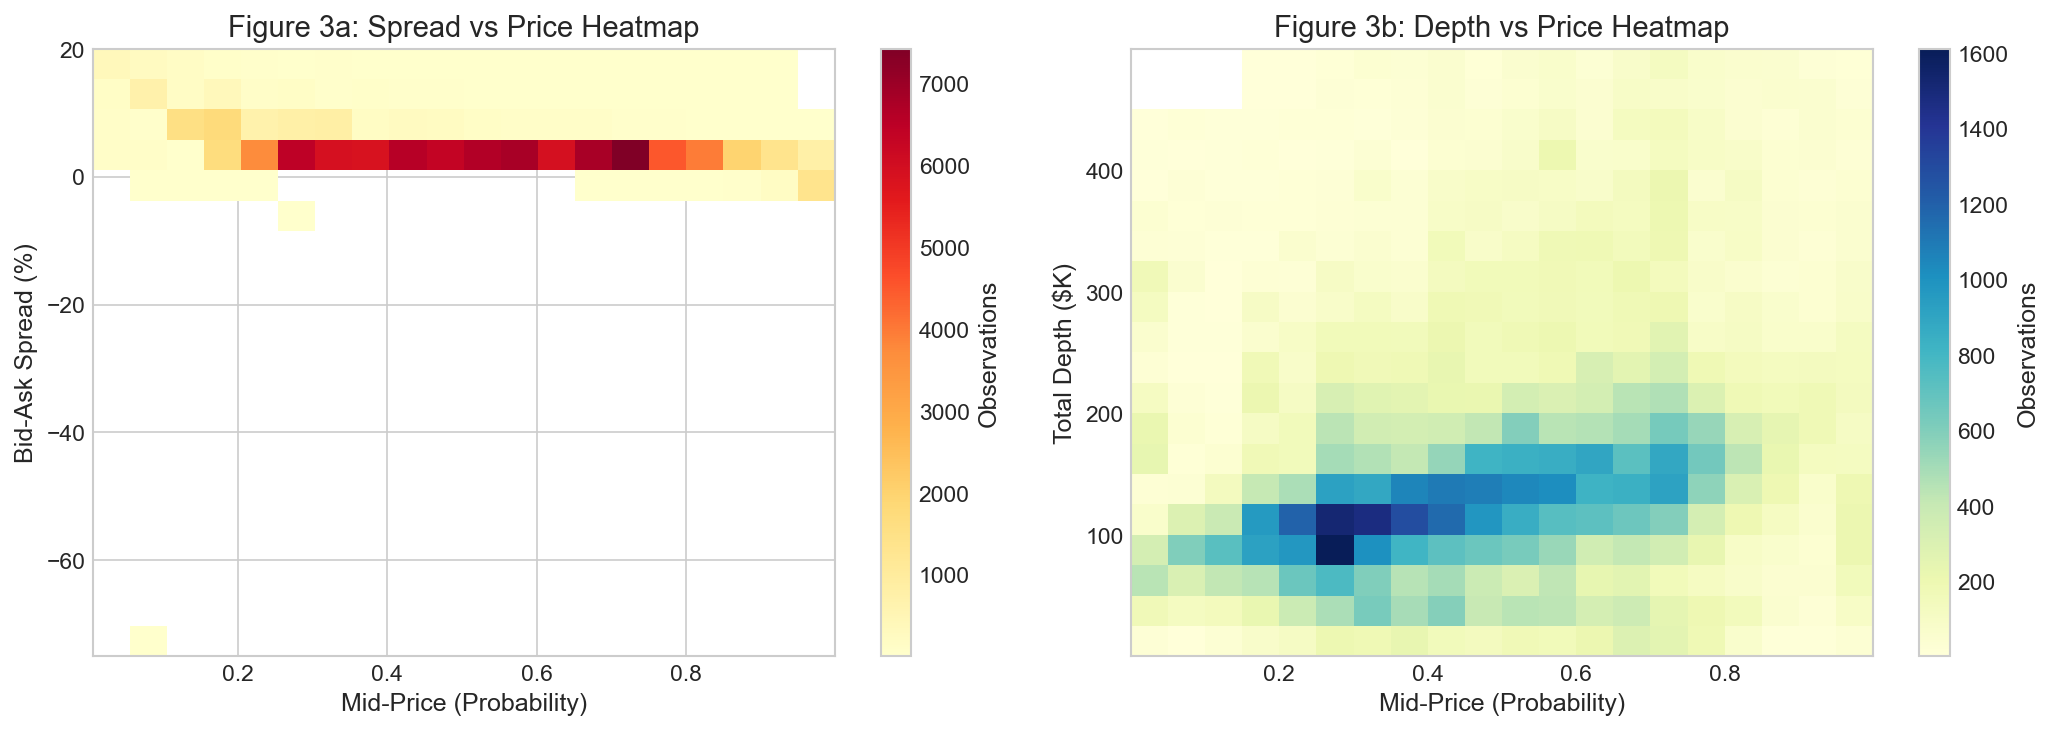
\includegraphics[width=0.78\textwidth]{figures/fig03_liquidity_heatmap.png}
\caption{Liquidity concentration heatmap by price level (vertical axis) and time of day (horizontal axis, Eastern Time). Darker colors indicate higher depth. Liquidity concentrates at mid-probability levels (40\%--60\%) during US evening hours (7--11 PM), creating optimal trading conditions in this region. Extreme probabilities and off-peak hours show substantially thinner depth.}
\label{fig:liquidity-heatmap}
\end{figure}

The heatmap reveals a clear liquidity ``sweet spot'' at the intersection of mid-range probabilities (40\%--60\%) and peak hours (7--11 PM Eastern). This region offers depths 2--3x higher than other areas, tighter spreads, and faster quote updates. Traders seeking optimal execution should concentrate activity in this zone when possible.

Liquidity deteriorates predictably in two dimensions. Vertically, moving toward extreme probabilities (below 20\% or above 80\%) reduces available depth by approximately 60\% relative to mid-range. Horizontally, trading outside the 7--11 PM window reduces depth by approximately 50\%. The combination of extreme probability and off-peak hours creates especially challenging execution conditions, with depths sometimes falling below \$10,000.

%------------------------------------------------------------------------------
% 3.5 Spread Determinants
%------------------------------------------------------------------------------
\section{Spread Determinants}

To understand what drives spread variation, we analyze relationships between spreads and potential determinants: probability level, depth, time of day, and game phase. Table~\ref{tab:spread-regression} summarizes these relationships.

\begin{table}[H]
\centering
\caption{Spread Determinants: Correlation Analysis}
\label{tab:spread-regression}
\begin{tabular}{lcc}
\toprule
\textbf{Factor} & \textbf{Correlation with Spread} & \textbf{Effect Direction} \\
\midrule
Distance from 50\% & +0.43 & Extreme probs $\rightarrow$ wider \\
Total Depth & -0.38 & More depth $\rightarrow$ tighter \\
Off-Peak Hours & +0.31 & Night/morning $\rightarrow$ wider \\
Game Phase (late) & +0.22 & Near resolution $\rightarrow$ wider \\
Volatility & +0.28 & High vol $\rightarrow$ wider \\
\bottomrule
\end{tabular}
\end{table}

Distance from 50\% probability shows the strongest relationship (+0.43 correlation), confirming that spreads widen systematically at extreme probabilities. This relationship is nonlinear: spreads increase modestly between 50\% and 80\% probability but accelerate sharply above 90\% or below 10\%.

Depth exhibits an expected negative relationship (-0.38): markets with more depth feature tighter spreads, consistent with competitive dynamics where abundant liquidity compresses margins. This relationship suggests that trading larger-volume games (which tend to have greater depth) provides execution advantages beyond size capacity.

The off-peak hours effect (+0.31) reflects reduced market maker activity and wider risk premiums demanded during low-activity periods. Chapter~\ref{sec:temporal} provides detailed analysis of temporal patterns.

%------------------------------------------------------------------------------
% 3.6 Key Findings
%------------------------------------------------------------------------------
\section{Key Findings}

\begin{keyfindings}[Orderbook Structure]
\begin{enumerate}
    \item \textbf{Competitive Spreads:} Median bid-ask spread of 2.3\% (\CI{2.2\%}{2.4\%}) indicates mature market infrastructure with trading costs comparable to established prediction platforms.

    \item \textbf{Substantial Depth:} Median total depth of \$142K (\CI{\$140K}{\$145K}) supports meaningful order sizes without excessive market impact, enabling both retail and modest institutional participation.

    \item \textbf{Persistent Ask-Side Dominance:} Consistent negative depth imbalance (median -0.36) indicates structural selling pressure. Sell orders face thinner liquidity than buy orders.

    \item \textbf{Probability-Dependent Liquidity:} Spreads widen and depth thins at extreme probabilities (below 20\% or above 80\%). Mid-range probabilities offer optimal execution conditions.

    \item \textbf{Time-Sensitive Quality:} Liquidity peaks during US evening hours aligned with NBA game schedules. Trading outside this window incurs meaningfully higher costs.
\end{enumerate}
\end{keyfindings}

%------------------------------------------------------------------------------
% 3.7 Trading Implications
%------------------------------------------------------------------------------
\section{Trading Implications}

The orderbook structure analysis yields several practical recommendations for traders:

\textbf{Target Mid-Probability Markets:} When multiple games or positions offer similar expected value, prefer those with probabilities in the 40\%--60\% range. These markets offer tighter spreads, deeper liquidity, and better execution quality.

\textbf{Time Execution Carefully:} Concentrate trading activity during US evening hours (7--11 PM Eastern) when liquidity is deepest. Urgent trades outside this window should account for 30--50\% wider spreads in position sizing.

\textbf{Account for Spread Costs:} A 2.3\% median spread translates to 4.6\% round-trip cost before any market impact. Strategies must generate sufficient edge to overcome this friction. Short-term trading faces particularly high hurdles given these costs.

\textbf{Anticipate Asymmetric Execution:} Given ask-side depth dominance, buy orders typically execute more easily than sell orders. Consider this asymmetry when planning position exits, potentially allowing extra time or accepting wider prices for sell execution.

\textbf{Monitor Spread Widening:} Sudden spread widening often precedes significant price moves or reflects information arrival. Wide spreads at unexpected times may signal that informed participants are active, warranting caution for new entries.

These findings establish the baseline execution environment for subsequent analyses. The following chapters examine how prices evolve within this liquidity structure (Chapter~\ref{sec:price-dynamics}) and how trade flow interacts with orderbook depth (Chapter~\ref{sec:trade-flow}).
